%!TEX root=../../thesis_rui_almeida.tex

\section{DOAS}%
\label{sec:doas}

Differential Optical Absorption Spectroscopy is a well established
absorption technique that is widely used in the field of atmospheric
studies~\cite{Platt2007}. In this section, I present a short
introduction to the field, extracted from~\cite{ValentedeAlmeida2017},
an article we have published in 2017, marking the conclusion of the
initial studies for this PhD thesis.

DOAS itself is based on Lambert--Beer's law, which can be written as
\cite{Platt2007}

\begin{equation}
  \centering
  \label{eq:lambertBeer}
  I(\lambda) = I_0 (\lambda) \cdot \exp(-\sigma(\lambda) \cdot c \cdot L) \;,
\end{equation}

Where $\lambda$ is the wavelength of the emitted light; $I(\lambda)$ is
the light intensity as measured by the system; $I_{0}(\lambda)$ is the
intensity of the light as emitted by the source; and $\sigma(\lambda)$
is the absorption cross section of absorber, which is wavelength
dependent; $c$ is the concentration of the absorber we want to measure.

This law allows the definition of optical thickness
($\tau$)~\cite{Platt2007}:

\begin{equation}
      \label{eq:opticalThickness}
      \tau(\lambda) = \ln \bigg( \frac{I_{0}(\lambda)}{I(\lambda)}\bigg)
      = \sigma(\lambda) \cdot c \cdot L.
\end{equation}

In a laboratory setting, Eq.~(\ref{eq:lambertBeer})
or~(\ref{eq:opticalThickness}) can be used to directly calculate an
absorber's concentration, provided there is knowledge of  its cross
section. In the open atmosphere, however, absorption spectroscopy
techniques are far more complex. On one hand, $I_0(\lambda)$ is not
accessible since we measure from inside the medium we want to measure.
On the other hand, there are several environmental and instrumental
effects that influence measurement results. These effects include the
following~\cite{Platt2007}.

\begin{itemize}
      \item Rayleigh scattering is due to small molecules present in the
          atmosphere and is heavily influenced by wavelength (hence the
          blue colour of the
      sky).
      \item Mie scattering is caused by particles and larger molecules
          suspended in the atmosphere and is not very dependent
      on the wavelength (hence the white colour of clouds).
      \item Instrumental and turbulence effects are the instrument's
          transmissivity and atmospheric turbulence in the optical path
          also limit light intensity.
  \end{itemize}

In addition, we also have to take into account that, in the atmosphere,
there are a number of trace gases that interfere with passing light.

Another aspect worth mentioning is that our device is never pointed
directly at the light source (the Sun) but always processes light that
has been scattered at some unknown point in the optical path. This means
that the light that reaches our detector is only the scattered fraction
of the sunlight, depending on the system's position and geometry, as
well as wavelength.

The expansion of Lambert--Beer's equation to include all these effects
results in Eq.~(\ref{eq:expandedLambertBeer}).

\begin{equation}
    \label{eq:expandedLambertBeer}
    \begin{aligned}
        \epsilon_\mathrm{\small{TG}}(\lambda, s)&=\sum_{i} \sigma_{i}(\lambda, s)
            \cdot c_{i}(s)\\
       I(\lambda) &= I_0(\lambda) \cdot A(\lambda, \ldots) \cdot
            S(\lambda) \cdot\\
                   &\quad\cdot \exp \left[ -\int \left[
                       \epsilon_{TG}(\lambda, s) +
                           \epsilon_{\mathrm{M}}(\lambda, s) +
                               \epsilon_{\mathrm{R}}(\lambda, s)  \right] \right] 
    \end{aligned}
\end{equation}

Where $A(\lambda, \ldots)$ is the fraction of scattered light that
reaches the device, $S(\lambda)$ represents instrumental and turbulence
effects, $\sigma_{i}(\lambda, s)$ is the absorption cross section of
absorber $i$, $c_{i}$ is the concentration of absorber $i$.
$\epsilon_{\mathrm{TG}}(\lambda, s)$ is the absorption by the $i$ trace gases,
$\epsilon_\mathrm{R}(\lambda, s)$ represents Rayleigh's extinction
coefficient and $\epsilon_\mathrm{M}(\lambda, s)$ represents Mie's
extinction coefficient.

The interest of this equation lies within the retrieval of $c_i$, a
given absorber's concentration. Since the integral is taken along the
total atmospheric path of the measured photons, and considering that
their cross sections do not vary significantly in atmospheric
conditions, it is possible to define the concept of slant column, which
is of great importance~\cite{Merlaud2013}.

\begin{equation}
      \label{eq:slantColumn}
      \mathrm{SC}_{i} = \int c_{i}(s)\mathrm{d}s
\end{equation}

This quantity, as Eq.~(\ref{eq:slantColumn}) shows, equals the integral
of an individual absorber's concentration along the atmospheric optical
path of relevance.

Now, without knowledge of $I_{0}(\lambda)$, these equations cannot give
us absolute concentration values. We can, however, use another scattered
light spectrum as reference in Eq.~(\ref{eq:opticalThickness}). Instead
of absolute densities, this will yield relative changes in the
atmosphere. We thus arrive at Eq.~(\ref{eq:relativeOpticalThickness}).

\begin{equation}
    \label{eq:relativeOpticalThickness}
    \begin{aligned}
        \ln\Bigg( \frac{I_\mathrm{ref}}{I}(\lambda) \Bigg) &= 
            \ln\Big( \frac{A_\mathrm{ref}}{A}(\lambda,\ldots) \Big) + \ln\Big( 
                \frac{S_\mathrm{ref}}{S}(\lambda) \Big) \nonumber\\
                                                           &+  \sum_{i} 
            (\sigma_{i}(\lambda) \cdot \Delta \mathrm{SC}_{i}(\lambda)) + 
                \Delta \tau_\mathrm{M}(\lambda) \nonumber\\
    \end{aligned}     
\end{equation}

Where $\Delta \mathrm{SC}_{i}$  is the relative slant column of absorber
$i$; $\Delta \tau_\mathrm{M}$  is the relative Mie scattering term,
integrated to its optical thickness; and $\Delta \tau_\mathrm{R}$ is the
relative Rayleigh scattering term, integrated to its optical thickness.

This is where the principle of DOAS is applied. Instrument features,
scattering and other atmospheric effects have broad absorption spectral
profiles, which vary slowly with wavelength. Several trace absorbers
have narrow and rapidly varying spectral signatures in at least a small
section of the spectrum. By using Eq.~(\ref{eq:separation}), we can
separate these contributions \cite{Danckaert2015}.

\begin{equation}
      \label{eq:separation}
      \sigma(\lambda) = \sigma{'}(\lambda) + \sigma_{0}(\lambda)
\end{equation}

Here, the broad part of the optical thickness ($\sigma_{0}(\lambda)$)
can be separated from the narrow part ($\sigma{'}(\lambda)$ --
differential) by approximating it by a low-order polynomial, resulting
in Eq.~(\ref{eq:DOAS}).

\begin{equation}
    \label{eq:DOAS}
    \begin{aligned}
        \ln\left( \frac{I_\mathrm{ref}}{I}(\lambda) \right) &= \sum_{i = 1}^{n} \sigma_{i}{'}(\lambda) 
            \cdot \Delta \mathrm{SC}_{i} + \sum_{j = 0}^{m} a_{j} \cdot \lambda^{j}
    \end{aligned}
\end{equation}

Where $\sum_{i = 1}^{n} \sigma_{i}{'}(\lambda) \cdot \Delta SC_{i}$ is
the differential part (narrowband, rapidly varying with wavelength) and
$\sum_{j = 0}^{m} a_{j} \cdot \lambda^{j}$ is a low-order polynomial,
used to remove the broadband spectral features resulting from
atmospheric and instrumental phenomena.

In practice, the mathematical solving of Eq.~(\ref{eq:DOAS}) is not
enough since it does not account for the Ring effect or the
non-linearities that result from stray light and wavelength shift in
measured and cross-section spectra.

The Ring effect is a consequence of rotational Raman scattering:
molecules in the atmosphere do not absorb photons in a purely elastic
(Rayleigh scattering) fashion. A small portion of the light--matter
interaction is in fact inelastic \cite{Brinkmann1968,Merlaud2013}. This
changes the light source frequencies as seen from the detector. This
phenomenon was first noticed by Grainger and Ring in 1962. At the time,
they noticed that the well-known Fraunhofer lines would slightly change
when one  observed them by using moonlight instead of scattered daylight
\cite{GRAINGER1962}. Mathematically, the Ring effect is introduced into
the \gls{DOAS} expressions as a synthetically produced pseudo-absorber.

Up until this point, the \gls{DOAS} problem can be solved by a system of
linear equations of the form displayed in
Equation~\ref{eq:linearSystem}.

\begin{equation}
    \label{eq:linearSystem}
    \tau = A \cdot X
\end{equation}

$A$ is an $m \times n$ matrix. Its columns are the differential
cross-sections fot he measurement target gas, $\sigma_{i}^{'}(\lambda)$,
and the wavelength powers ($\lambda$ ,$\lambda^2$, $\lambda^3$, \ldots)
according to the polynomial used for the broadband extraction described
above, $P(\lambda)=\sum_{j=0}^{m} a_{j}\lambda^{j}$. The lines of matrix
$A$ are the wavelength window of study, as \emph{seen} by the
spectrometer used in the experiment. This leads to there being many more
lines than columns in $A$. The system is thus overdetermined. Solving it
requires the use of numerical approximations, and the most common
approach is a least-squares approximation, in which the best solution
minimises $\chi^2=\left[\tau - A \cdot X\right]\left[\tau - A \cdot
X\right]^T$. The upper script $T$ used in this expression denotes the
transpose of the preceding matrix.

A crude \gls{DOAS} algorithm might not go any forward. In effect, this
is precisely the approached followed in~\cite{ValentedeAlmeida2017} for
smoke detection using machine learning techniques. A more refined
measurement, aimed at quantification of the target trace gases and not
at determining the presence of a particular type of atmospheric event
requires an additional consideration, and some more algorithmic steps.
There are in fact some non-linearities in the complete retrieval
process. These non-linearities are not retrievable through linear
algorithms alone. These non-linear effects present themselves as shifts,
stretches and offsets in the measured signal. They do not directly
change the dependent variable values (i.e., the radiance), but instead
"move" the scale of the independent variable (i.e., the wavelength).
Therefore, linear approximations such as least-squares minimisation are
not sensitive to them. A non-linear approximation algorithm such as
Levenberg--Marquardt~\cite{Press2007} can be used, and the expression
that is being solved is presented in Equation~\ref{eq:DOAS_nonLinear}.

\begin{equation}
    \label{eq:DOAS_nonLinear}
    \begin{aligned}
        \ln \left( \frac{I_\mathrm{ref}(\lambda)}{I(\lambda +
            \mathrm{shift}) + \mathrm{offset}} \right) &= \sum_{i=1}^{n}
                \sigma_{i}{'}(\lambda) \cdot \Delta \mathrm{SC}_{i} + 
                    \sum_{j=0}^{m} a_{j} \cdot \lambda^{j}
    \end{aligned}
\end{equation}

Programming-wise, solving these equations is an iterative two-stage
process, which runs until one of the following typical stop criteria are
met.

\begin{description}
    \item[Maximum iteration number:] This is a self-explanatory
        criterion. It limits the number of times the algorithm's cycle
        can run; 
    \item[Minimum improvement threshold:] As the algorithm proceeds,
        this criterion ensures that it progresses in the correct
        direction, i.e., minimising $\chi^2$;
    \item[Minimisation target:] If $\chi^2$ becomes lower than this
        given threshold, the cycle is terminated. 
\end{description}

The cycle begins by the determination of the concentration values of the
target trace gases and the $\chi^2$ score is calculated. The wavelength
window is shifted, stretched and offset according to the initial
conditions. The $\chi^2$ is re-calculated and compared to the previous
value. This cycle is iteratively repeated in the best minimisation
direction until any of the stop criteria are met and the cycle is
terminated. Algorithm~\ref{alg:doas_non_linear} summarises this process.

\missingfigure{DOAS non linear}

There are two main families of \gls{DOAS} assemblies, with different
goals and capabilities:

\begin{itemize}

        \item Active systems, of which a simple illustration is
            presented in Fig.~\ref{fig:activeSmall}, are characterized
            by relying on an artificial light source for their
            measurements. A spectrometer at the end of the light path
            performs spectroscopic detection. Active DOAS techniques are
            very similar to traditional in-lab absorption spectroscopy
            techniques \cite{Platt2007};

            \begin{figure}[htb]
                \centering
                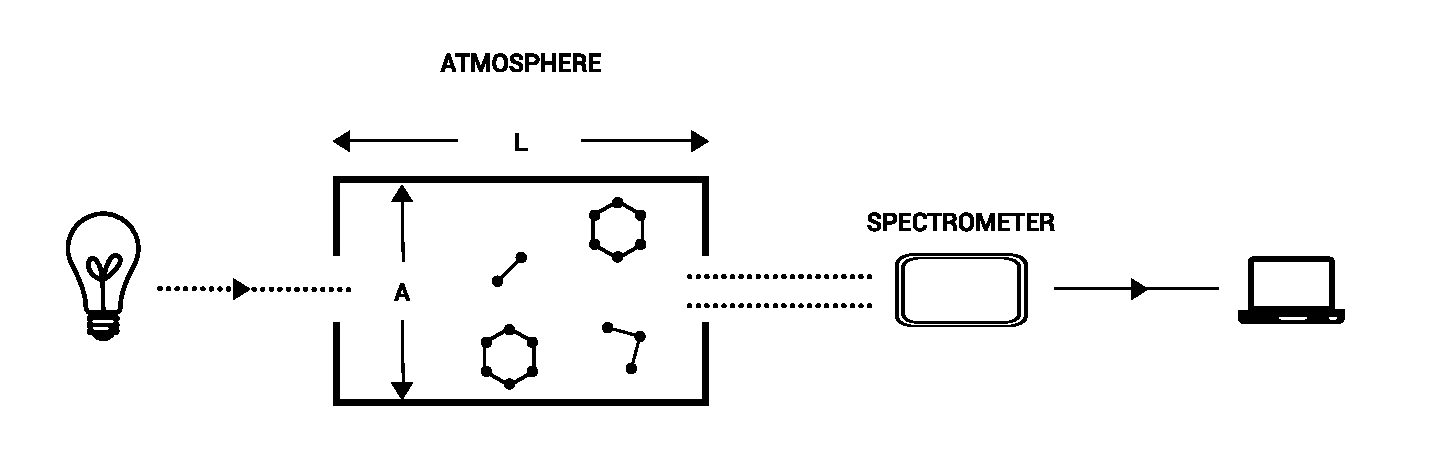
\includegraphics[width=.8\textwidth]{img/pdf/amt-2016-314-f02.pdf}
                \caption{Active DOAS schematic.}\label{fig:activeSmall}
              \end{figure}


        \item Passive DOAS techniques, illustrated in
            Fig.~\ref{fig:passiveSchematic}, use natural light sources,
            such as the Sun and the moon, in their measurement process.
            An optical system is pointed in certain elevation and
            azimuth angles and sends the captured light into a
            spectrometer, connected to a computer. The system returns
            the total value of the light absorption in its
            path~\cite{Platt2007,Merlaud2013}.

              \begin{figure}[htb]
                  \centering
                  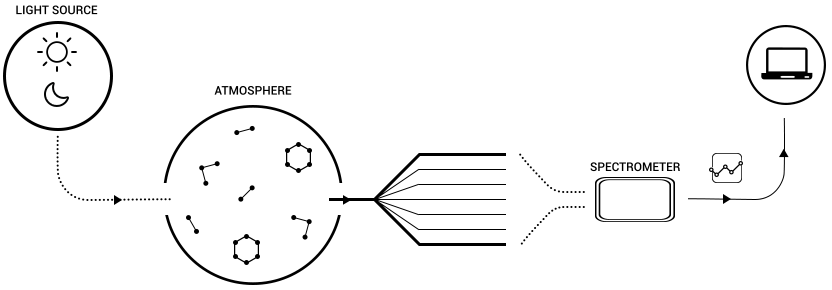
\includegraphics[width=.8\textwidth]{img/png/amt-2016-314-f03.png}
                  \caption{Passive DOAS schematic.}\label{fig:passiveSchematic}
              \end{figure}

\end{itemize}

\todo[inline]{MISSING}
\begin{itemize}
    \item types of active and passive measurements
    \item scattered sunlight measurements;
    \item satellite based measurements (SCIAMACHY).
\end{itemize}
